\begin{figure}[h]
    \centering
    \begin{minipage}[c]{0.3\textwidth}
        \centering
        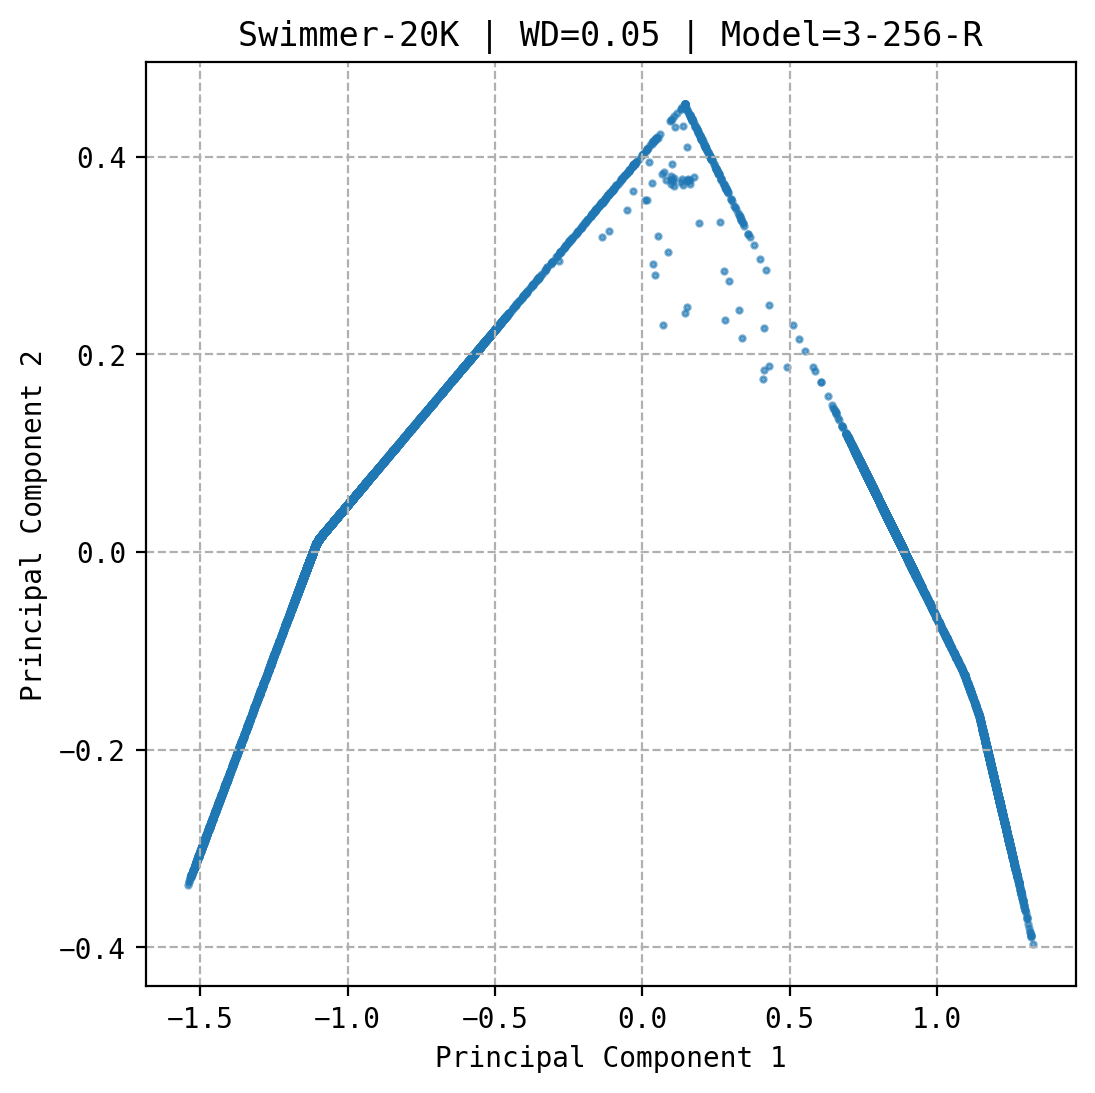
\includegraphics[width=\linewidth]{figures/Main_body/feature_pca_swimmer20K.png}
    \end{minipage}
    \hfill
    \begin{minipage}[c]{0.318\textwidth}
        \centering
        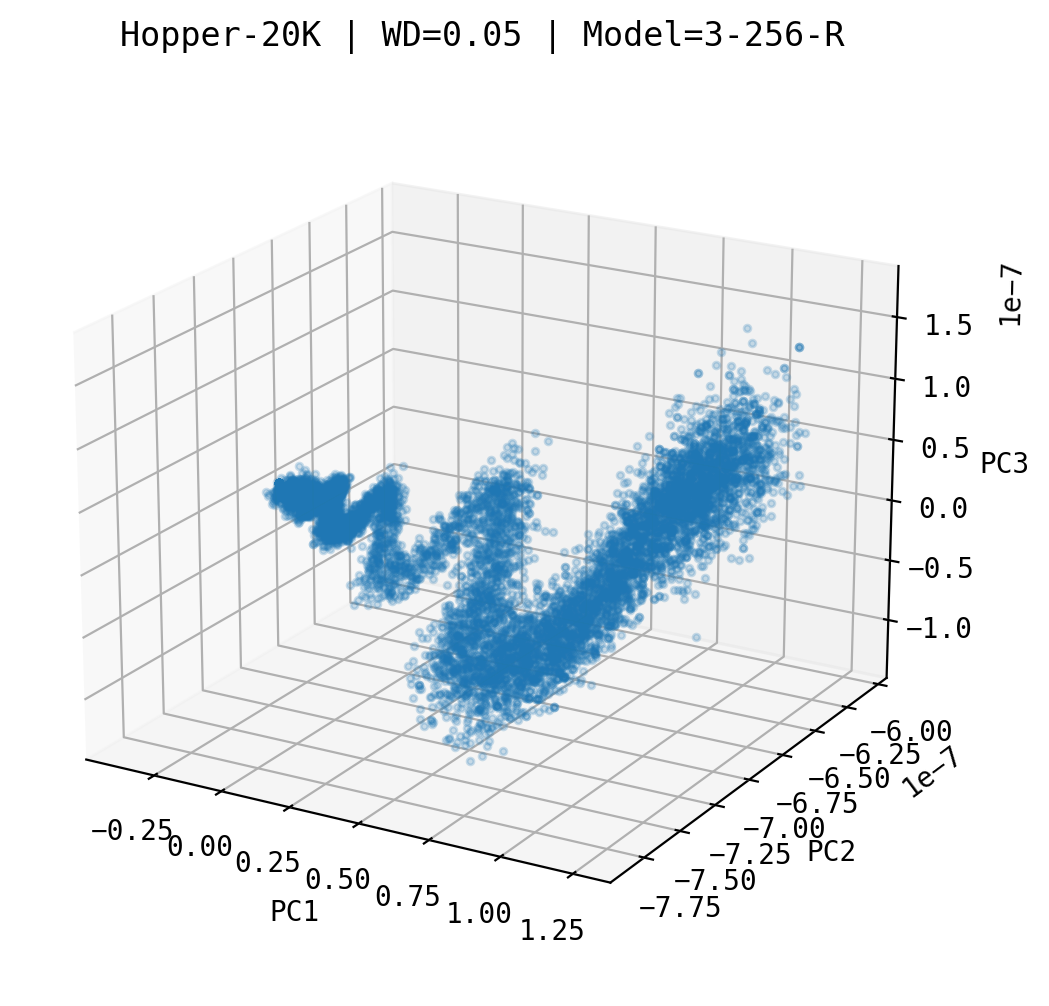
\includegraphics[width=\linewidth]{figures/Main_body/feature_pac_hopper20K.png}
    \end{minipage}
    \hfill
    \begin{minipage}[c]{0.31\textwidth}
        \centering
        % \vspace{0pt}
        \small
        \begin{tabular}{ccc}
            \toprule
            $k$ & Global PCA & Local PCA \\
            \midrule
            6 & $3.4\!\times\!10^{-3}$ & $2.8\!\times\!10^{-5}$ \\
            5 & $7.5\!\times\!10^{-3}$ & $7.9\!\times\!10^{-5}$ \\
            4 & $8.4\!\times\!10^{-2}$ & $3.5\!\times\!10^{-4}$ \\
            3 & $4.9\!\times\!10^{-1}$ & $1.5\!\times\!10^{-3}$ \\
            \bottomrule
        \end{tabular}
    \end{minipage}
    \caption{Nonlinear structure of collapsed feature manifolds. \textbf{Left, Center:} PCA projections of collapsed 1D feature manifolds for Swimmer ($n=2$) and Hopper ($n=3$), showing visibly curved structures. \textbf{Right:} Global vs.\ local PCA projection error for collapsed Halfcheetah features ($\idh = 3.6$, $n=6$). Local errors (projection onto the top-$k$ PCs of 64-nearest-neighbor feature matrix) are orders of magnitude smaller, confirming locally flat but globally curved geometry.}
    \label{fig:nonlinear_manifold}
\end{figure}